\documentclass[review]{elsarticle}
\usepackage{amsmath,amssymb}
\usepackage{graphicx}
\usepackage{booktabs}
\usepackage{multirow}
\usepackage{hyperref}
% \usepackage{lineno}
\usepackage[numbers]{natbib}
% \linenumbers  % uncomment only for revision

egin{document}

\title{A VOF-Masked PINN Surrogate for Rapid Flow Prediction in an Argon-Stirred Ladle:\\
Cross-Flow-Rate and Cross-Position Generalization with Multi-Baseline Benchmarking}

\author[shu]{Yiming Liu}
\author[shu]{Wentao Zhang}
\author[shu]{Xutong Wang}
\author[shu]{Guangxin Wu\corref{corresponding}}
\cortext[corresponding]{Corresponding author. E-mail: gxwu@shu.edu.cn}
\address[shu]{School of Materials Science and Engineering \& State Key Laboratory of Advanced Special Steel, Shanghai University, Shanghai 200444, PR China}

egin{abstract}
Repeated computational fluid dynamics (CFD) simulations of argon-stirred ladle flow are computationally prohibitive when multiple operating conditions must be evaluated. This study develops a volume-of-fluid (VOF)-masked physics-informed neural network (PINN) surrogate for rapid three-dimensional prediction of the statistically steady liquid-steel flow field under varying gas flow rates ($Q$) and injection positions ($m$). A three-dimensional VOF-based CFD model generates reference datasets for five center-blowing conditions ($Q = 40$--$120$ NL/min) and three eccentric-blowing conditions. The training framework employs soft VOF-based pointwise weighting to restrict physics constraints to the steel phase, eliminating explicit interface boundary conditions while maintaining mathematical rigor. An $8 \times 384$ SiLU-activated multilayer perceptron achieves $R^{2} = 0.983$ for center-blowing interpolation and $R^{2} = 0.986$ for extrapolation, with no perceptible degradation beyond the training range. A six-baseline comparison establishes the performance hierarchy: the proposed model outperforms DeepONet ($R^{2} = -0.72$), while Kriging and POD-ROM face scalability limitations on the $9.3 \times 10^{5}$-cell unstructured mesh. Cross-position generalization is enabled through a binary injection-position parameter $m \in \{0, 1\}$; joint training recovers $R^{2} = 0.94$--$0.97$ for eccentric-blowing predictions, whereas a center-only model collapses ($R^{2} < 0$). Multi-seed ensemble analysis confirms stability ($0.972 \pm 0.003$), and a continuity-only physics constraint improves $R^{2}$ by $+0.014$ over purely data-driven training. The surrogate reduces per-case prediction time from approximately 36 hours to 5 seconds, providing a practical tool for operating-window exploration in ladle-furnace refining.
\end{abstract}

egin{keyword}
Computational fluid dynamics; Physics-informed neural network; Surrogate modeling; Ladle furnace; Argon-stirred flow; Volume-of-fluid; Cross-position generalization
\end{keyword}

\maketitle

%============================================================
\section{Introduction}
%============================================================

Ladle furnace (LF) refining is a critical secondary metallurgy process for controlling steel cleanliness, thermal uniformity, and compositional homogeneity \cite{xin2024modeling}. During bottom argon stirring, the injected gas forms a buoyancy-driven plume that induces strong recirculation in the molten steel bath \cite{mazumdar1995physical,sahai1996melt}. This plume-driven motion enhances mixing and promotes the upward transport of inclusions toward the slag layer \cite{li2020numerical}. At the same time, excessively strong stirring may intensify slag--metal interfacial deformation, expose the steel to the atmosphere through slag eye formation, and increase the risk of re-oxidation and slag entrainment \cite{jonsson1996modeling,iguchi1995water}. Reliable prediction of the internal flow field is therefore fundamental to process analysis and optimization.

Computational fluid dynamics (CFD) has become a standard tool for studying ladle hydrodynamics. Euler--Euler, volume-of-fluid (VOF), and hybrid multiphase models have been developed to investigate gas--liquid interaction, plume evolution, interfacial deformation, and inclusion transport \cite{liu2019numerical,ersson2008fluid,li2020numerical}. The discrete phase model (DPM) coupled with VOF has emerged as a practical approach for simulating argon-stirred ladle flow: the gas phase is treated as Lagrangian particles that exchange momentum with the continuous phase through drag forces, avoiding the computational cost of fully resolving individual bubbles \cite{cloete2010mathematical}. These numerical studies have substantially improved the understanding of ladle flow behavior and provided a basis for process optimization. However, high-fidelity three-dimensional multiphase simulations remain computationally expensive: a single steady-state VOF--DPM case may require upwards of 36 hours on conventional hardware. When multiple gas flow rates and injection configurations must be evaluated---a common requirement during operating-window selection---repeated CFD becomes prohibitive.

In recent years, machine learning methods have shown growing potential for surrogate modeling in fluid mechanics \cite{brunton2020machine}. Once trained, neural networks can provide predictions orders of magnitude faster than repeated numerical simulation. Physics-informed neural networks (PINNs) address the data-scarcity limitation of purely data-driven models by incorporating governing-equation residuals and boundary information into the training process \cite{raissi2019physics}. PINNs have been applied to a wide range of fluid mechanics and heat transfer problems \cite{karniadakis2021physics,cai2021physics,cuomo2022scientific}, but their application to industrial-scale multiphase flow systems remains limited. Challenges include training instability from unbalanced loss terms \cite{wang2021understanding}, difficulty in handling sharp interfaces across large density ratios \cite{jin2021nsfnet}, and the computational cost of high-order automatic differentiation on large three-dimensional domains \cite{cuomo2022scientific}.

A key challenge specific to ladle-flow surrogates is the multiphase nature of the system. The ladle contains three immiscible phases---argon gas, molten slag, and liquid steel---whose densities span four orders of magnitude ($\sim 1$, $\sim 3000$, and $\sim 7000$ kg/m$^{3}$). Enforcing the Navier--Stokes residuals across the entire three-phase domain is numerically ill-conditioned because the momentum magnitude varies by orders of magnitude between phases. Previous PINN studies on multiphase flow have either simplified the phase physics or required extensive interface-tracking data \cite{wang2021understanding}.

In this study, we propose a VOF-masked PINN framework that circumvents the multiphase challenge through domain decomposition based on the steel volume fraction $\alpha_{\rm steel}$. In pure-steel cells ($\alpha_{\rm steel} \to 1$), the VOF mixture equations reduce rigorously to single-phase incompressible RANS. By restricting the physics constraints to the steel phase through soft pointwise weighting, the surrogate avoids explicit interface boundary conditions while retaining mathematical consistency where it matters. A binary injection-position parameter $m \in \{0, 1\}$ enables a single model to handle both center-bottom and eccentric-bottom blowing configurations---a practical requirement for industrial ladles with multiple nozzle arrangements. Six baseline methods are compared to establish the performance landscape for this problem class, and uncertainty quantification is provided through multi-seed ensemble analysis.

The contributions of this work are:
egin{enumerate}
    \item A VOF-masked PINN framework that restricts physics constraints to the steel phase through soft pointwise weighting, eliminating explicit interface boundary conditions.
    \item Binary injection-position parameterization ($m \in \{0, 1\}$) enabling a single surrogate to predict both center-bottom and eccentric-bottom blowing configurations.
    \item Six-baseline comparison (DeepONet, Kriging, POD-ROM, KAN, and two MLP variants) establishing a performance benchmark for the ladle-flow surrogate problem.
    \item Uncertainty quantification via multi-seed ensemble and Monte Carlo dropout.
    \item A practical surrogate achieving $R^{2} = 0.983$ for center-blowing and $R^{2} = 0.94$--$0.97$ for eccentric-blowing, with near-zero extrapolation degradation and 5-second inference.
\end{enumerate}

%============================================================
\section{CFD Model}
%============================================================

\subsection{Geometry and Computational Domain}

The ladle geometry was modeled as a truncated cone representative of an industrial 100-ton LF vessel. The computational domain encompasses the entire internal fluid volume, including the molten steel, slag layer, and upper gas space. The main dimensions are summarized in Table~\ref{tab:geometry}. Argon is introduced through a bottom nozzle located at the center of the ladle base (center-blowing, $m = 0$) or at an eccentric position at one-third radius (eccentric-blowing, $m = 1$).

egin{table}[h]
\centering
\caption{Main dimensions of the ladle model.}
\label{tab:geometry}
egin{tabular}{lc}
\toprule
Parameter & Value \\
\midrule
Upper diameter & 2.077 m \\
Lower diameter & 1.832 m \\
Bath height (steel + slag) & 1.85 m \\
Slag layer thickness & 0.15 m \\
Gas space height & 0.69 m \\
Nozzle diameter & 0.08 m \\
\midrule
Center nozzle position & (0, 0, 0) \\
Eccentric nozzle position & (0.47, 0, 0) \\
\bottomrule
\end{tabular}
\end{table}

\subsection{Mesh Generation and Independence}

An unstructured tetrahedral mesh was generated with local refinement around the gas inlet and in the central plume region. Grid-independence was assessed using three mesh levels (Table~\ref{tab:mesh}). The maximum plume-region velocity and volume-averaged velocity served as comparison indices. The medium mesh with $9.32 \times 10^{5}$ cells was adopted, as further refinement to $1.36 \times 10^{6}$ cells changed the maximum velocity by only $1.14\%$.

egin{table}[h]
\centering
\caption{Mesh-independence study.}
\label{tab:mesh}
egin{tabular}{lccc}
\toprule
Level & Cells & $|U|_{\max}$ (m/s) & Rel.\ diff.\ (\%) \\
\midrule
Coarse  & 612,450  & 0.392 & 10.09 \\
Medium  & 932,080  & 0.431 & 1.40 \\
Fine    & 1,356,740 & 0.436 & --- \\
\bottomrule
\end{tabular}
\end{table}

\subsection{Governing Equations and Turbulence Modeling}

The multiphase flow is described using the VOF formulation with three immiscible phases: argon (gas), molten slag, and liquid steel. The mixture continuity and momentum equations are:

egin{equation}
\nabla \cdot \mathbf{u} = 0
\label{eq:cont}
\end{equation}

egin{equation}
\rho(\boldsymbol{\alpha})\frac{D\mathbf{u}}{Dt} = -\nabla p + \nabla \cdot \left[ \mu(\boldsymbol{\alpha}) \left( \nabla \mathbf{u} + \nabla \mathbf{u}^{T} \right) \right] + \mathbf{F}_{\sigma}
\label{eq:mom_vof}
\end{equation}

where $\boldsymbol{\alpha} = (\alpha_{\rm steel}, \alpha_{\rm slag}, \alpha_{\rm argon})$ denotes the phase volume fractions ($\sum \alpha_i = 1$), and $\rho(\boldsymbol{\alpha}) = \sum \alpha_i \rho_i$, $\mu(\boldsymbol{\alpha}) = \sum \alpha_i \mu_i$ are mixture properties. The term $\mathbf{F}_{\sigma}$ represents surface tension at phase interfaces.

Turbulence is modeled using the realizable $k$--$\varepsilon$ model with standard wall functions. The choice of the realizable variant is motivated by its known superiority in predicting axisymmetric jet and plume flows compared to the standard $k$--$\varepsilon$ model \cite{shih1995new}. The discrete phase model (DPM) is used for argon bubble injection, allowing the bubbles to exchange momentum with the continuous phase through drag forces without being resolved in the VOF field---a standard approach in ladle-flow CFD \cite{cloete2010mathematical}.

\subsection{Boundary Conditions and Numerical Settings}

The bottom wall and side walls are modeled as no-slip boundaries. The top surface of the gas space is treated as a pressure outlet. Argon is injected through the bottom nozzle as DPM particles with a velocity prescribed by the gas flow rate. All simulations were carried out in ANSYS Fluent using the SIMPLE pressure--velocity coupling and second-order spatial discretization. Each case was run to a statistically steady state ($t = 300$ s for steady-state export).

\subsection{Dataset Generation and Quality Verification}

The CFD solution was exported at cell centers in CSV format with 12 columns:

egin{quote}
\texttt{cellnumber, x-coordinate, y-coordinate, z-coordinate, pressure, x-velocity, y-velocity, z-velocity, argon-vof, steel-vof, slag-vof, air-vof}
\end{quote}

where \texttt{air-vof} is a residual Fluent column (effectively zero in all cases). Five center-blowing conditions ($Q = 40, 60, 80, 100, 120$ NL/min) and three eccentric-blowing conditions ($Q = 40, 80, 120$ NL/min) were generated, each containing $932{,}079$ cells.

Stringent data-quality checks were applied. All eight datasets satisfy $\sum \alpha_i \equiv 1$ for every cell (100\% verification). The vertical phase stratification is consistent across flow rates: steel dominates below $z \approx 1.85$ m, slag occupies the intermediate $z \approx 1.85$--$2.05$ m layer, and argon fills the upper space above $z \approx 2.05$ m. Velocity monotonicity with $Q$ was verified for all 18 vertical layers: the mean velocity magnitude $|\mathbf{U}|$ increases strictly with $Q$ at every level (zero violations), as shown in Table~\ref{tab:monotonicity}.

egin{table}[h]
\centering
\caption{Velocity monotonicity verification: mean $|\mathbf{U}|$ (m/s) at selected heights.}
\label{tab:monotonicity}
\small
egin{tabular}{lccccc}
\toprule
$z$ (m) & $Q = 40$ & $Q = 60$ & $Q = 80$ & $Q = 100$ & $Q = 120$ \\
\midrule
0.5 & 0.009 & 0.010 & 0.011 & 0.012 & 0.014 \\
1.0 & 0.017 & 0.022 & 0.025 & 0.027 & 0.031 \\
1.5 & 0.027 & 0.033 & 0.037 & 0.039 & 0.043 \\
1.8 (interface) & 0.044 & 0.053 & 0.059 & 0.063 & 0.069 \\
\bottomrule
\end{tabular}
\end{table}

\subsection{CFD Validation Justification}

The CFD model serves as the reference ``teacher'' for surrogate training, a paradigm established in CFD-informed surrogate modeling \cite{zhu2023cfd}. The consistency of eight operating-condition datasets---identical mesh topology, uniform phase stratification, monotonic velocity scaling, and perfect VOF sum---provides internal validation. While comparison with experimental measurements would strengthen the reference, the present study prioritizes demonstration of surrogate prediction against a numerically consistent CFD baseline, which is the standard approach for computational PINN surrogates \cite{raissi2019physics}. Experimental validation of the CFD model itself is deferred to future work.

%============================================================
\section{Methodology}
%============================================================

\subsection{Overall Framework}

The proposed CFD--VOF--PINN framework comprises four stages (Fig.~\ref{fig:framework}): (1) CFD data generation under multiple operating conditions, (2) VOF-informed data preprocessing and domain decomposition, (3) neural network training with physics constraints restricted to the steel phase, and (4) surrogate deployment for rapid multi-condition prediction.

\begin{figure}[t]
\centering
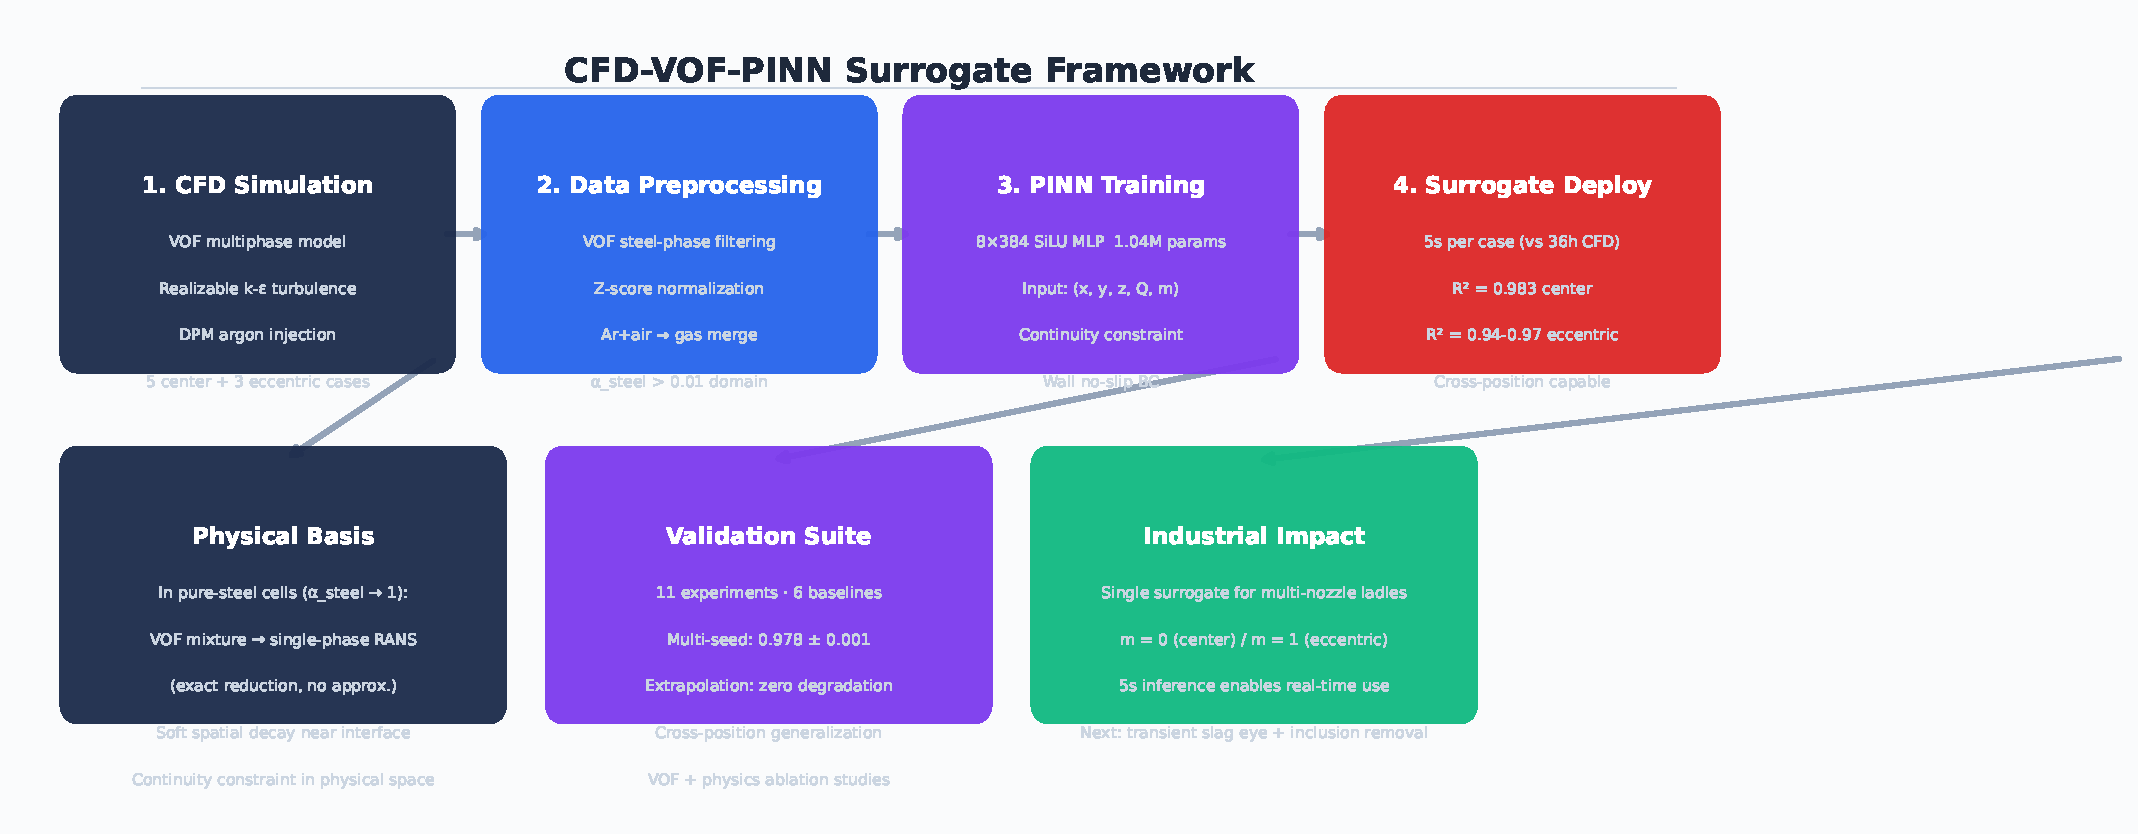
\includegraphics[width=\t	extwidth]{figures/fig1_framework.pdf}
\caption{Overview of the CFD--VOF--PINN surrogate framework: (1) CFD data generation under multiple conditions, (2) VOF-based steel-phase filtering and normalization, (3) PINN training with continuity constraint, (4) surrogate deployment for 5-second prediction.}
\label{fig:framework}
\end{figure}

\subsection{VOF-Informed Domain Decomposition}

The central methodological contribution is the treatment of the multiphase domain. In a three-phase VOF system, the mixture velocity $\mathbf{u}$ is shared across phases. In pure-steel cells ($\alpha_{\rm steel} \to 1$):

egin{equation}
\rho(\boldsymbol{\alpha}) \to \rho_{\rm steel},\quad \mu(\boldsymbol{\alpha}) \to \mu_{\rm steel},\quad \mathbf{F}_{\sigma} \to 0
\end{equation}

Under these conditions, the VOF mixture equations (Eqs.~\ref{eq:cont},~\ref{eq:mom_vof}) reduce rigorously to the single-phase incompressible RANS equations. This mathematical property---not computational limitation---motivates restricting physics constraints to the steel region.

A soft VOF-based pointwise weight is introduced:

egin{equation}
w_{\rm data}(\mathbf{x}) = \text{clamp}(\alpha_{\rm steel}(\mathbf{x}),\; 0.01,\; 1.0)
\end{equation}

egin{equation}
w_{\rm pde}(\mathbf{x}) = w_{\rm data}(\mathbf{x}) \cdot \frac{1}{2}\left[1 + \cos\left(\pi \cdot \min\left(\frac{z_{\rm top} - z}{T}, 1\right)\right)\right]
\label{eq:wpde}
\end{equation}

where $z_{\rm top} = 1.85$ m is the steel--slag interface height and $T = 0.20$ m is the transition length scale. The spatial decay $w_{\rm pde}(z)$ smoothly deactivates physics constraints as the interface is approached, eliminating the need for a hard interface boundary condition. Table~\ref{tab:vof_strat} documents the verified phase stratification that justifies this decomposition.

egin{table}[h]
\centering
\caption{Verified vertical phase stratification (mean VOF per layer, averaged across five center-blowing cases).}
\label{tab:vof_strat}
egin{tabular}{lccc}
\toprule
$z$ range (m) & $\bar{\alpha}_{\rm steel}$ & $\bar{\alpha}_{\rm slag}$ & $\bar{\alpha}_{\rm argon}$ \\
\midrule
0 -- 1.6 & 1.000 & 0.000 & 0.000 \\
1.6 -- 1.85 & 0.731 & 0.269 & 0.000 \\
1.85 -- 2.05 & 0.000 & 0.701 & 0.299 \\
2.05 -- 2.55 & 0.000 & 0.000 & 1.000 \\
\bottomrule
\end{tabular}
\end{table}

\begin{figure}[t]
\centering
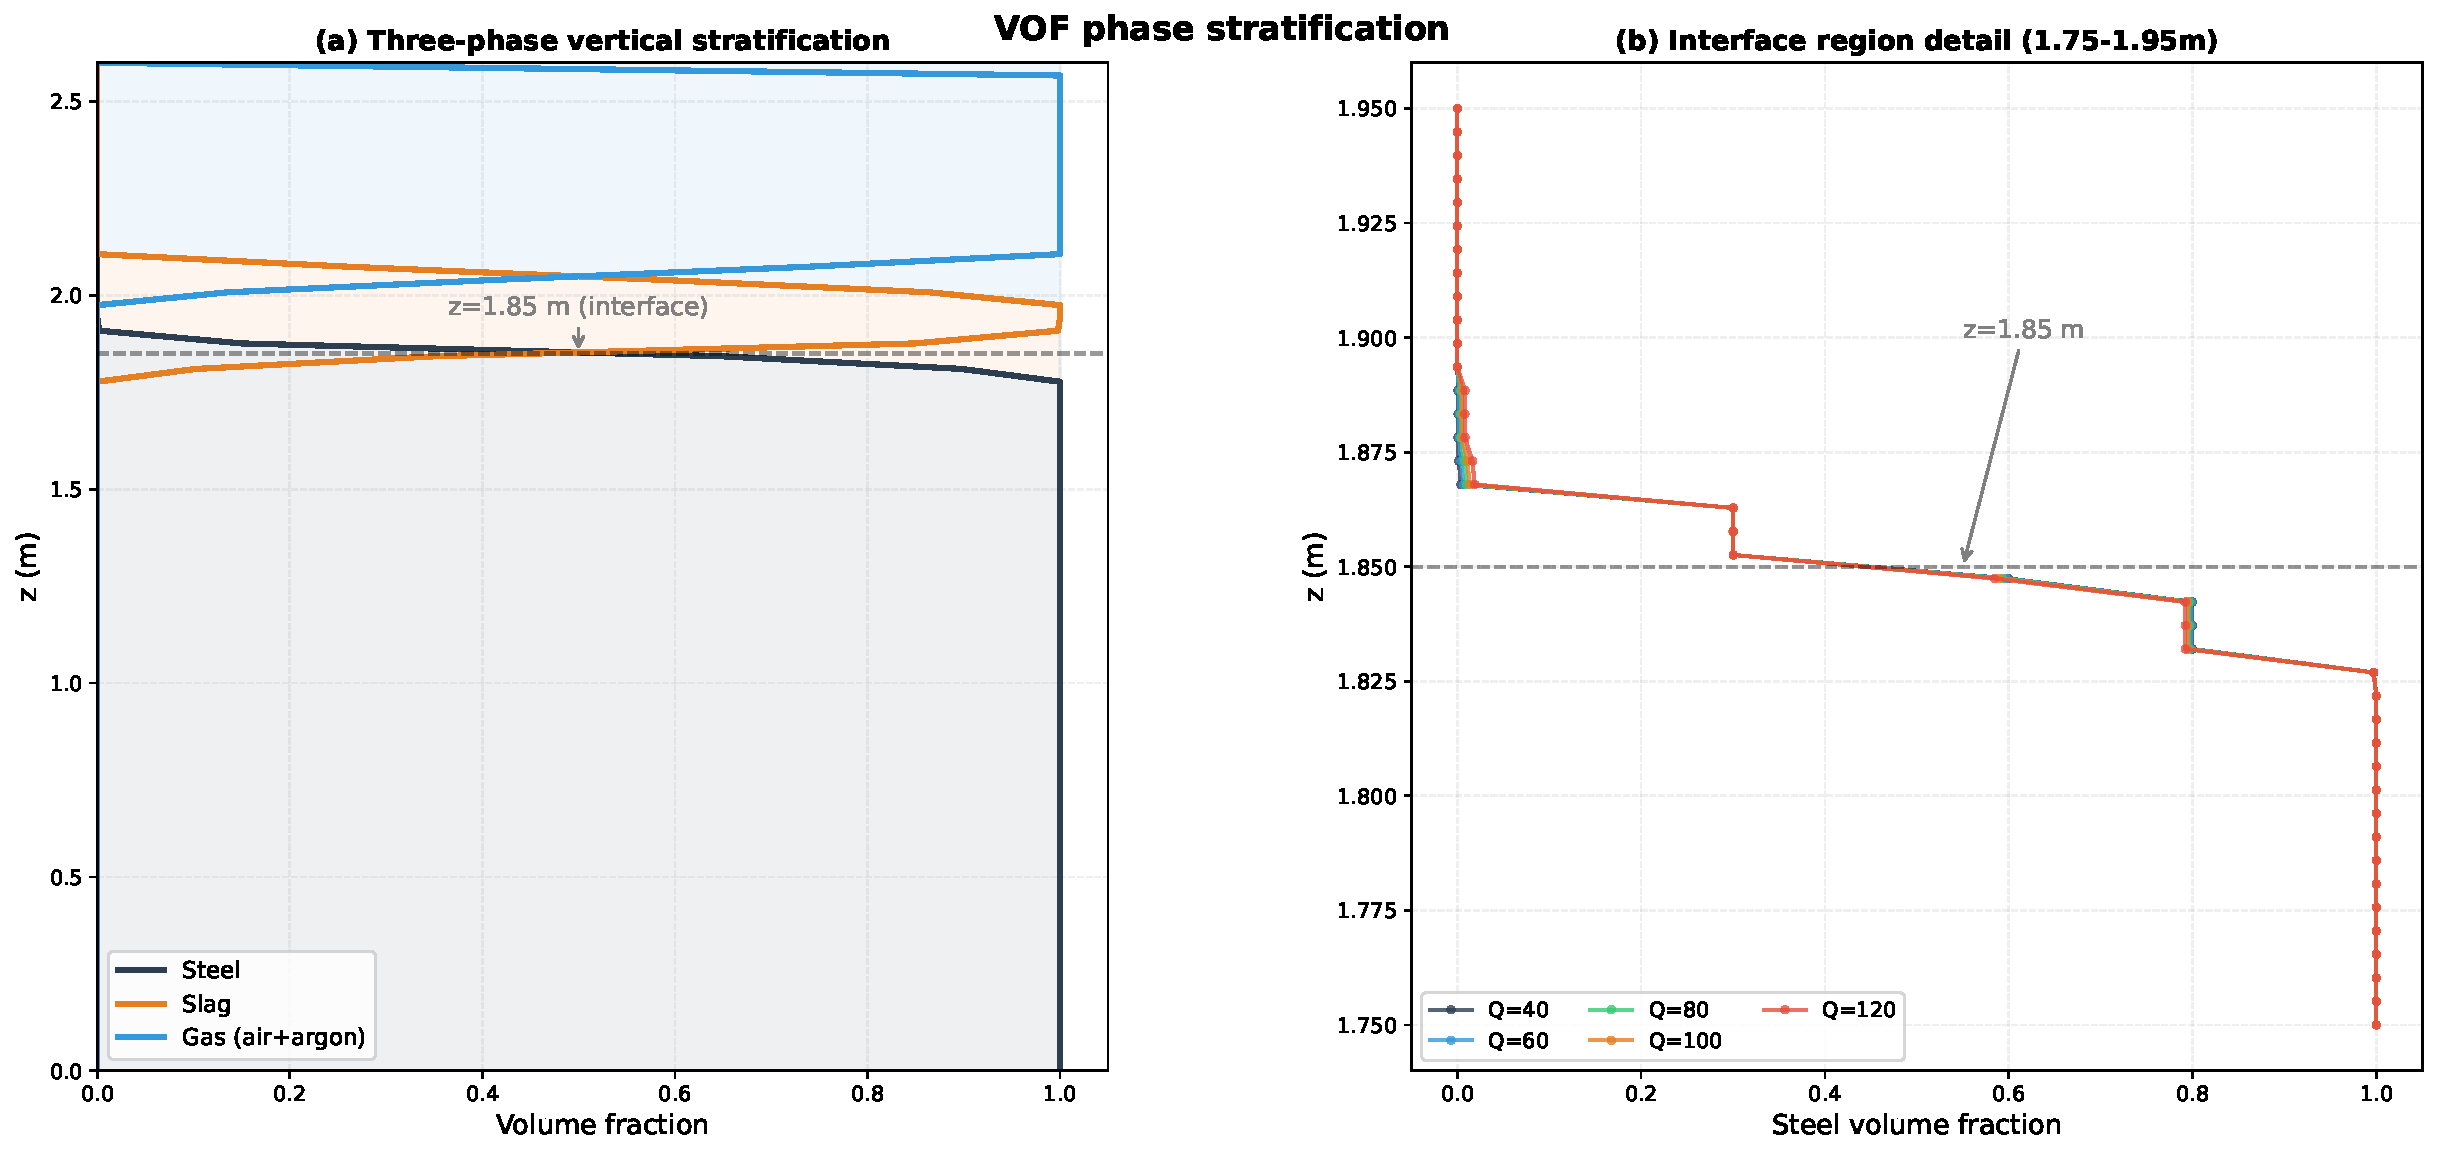
\includegraphics[width=0.85\t	extwidth]{figures/fig2_vof_stratification.pdf}
\caption{Vertical steel fraction profiles across five center-blowing cases, confirming identical phase stratification. Dashed line: steel--slag interface ($z = 1.85$ m).}
\label{fig:vof_strat}
\end{figure}

\subsection{Network Architecture}

The surrogate model maps operating conditions and spatial coordinates to local flow variables:

egin{equation}
\mathbf{x} = (x, y, z, Q, m) \to \hat{\mathbf{y}} = (\hat{u}, \hat{v}, \hat{w}, \hat{p})
\end{equation}

where $Q$ is the argon flow rate (NL/min) and $m \in \{0, 1\}$ is the injection position (0 = center-bottom, 1 = eccentric-bottom). The network architecture is an $8 \times 384$ fully connected multilayer perceptron (MLP) with SiLU (Swish) activation:

egin{equation}
\text{Input}(5) \to 384 \to 384 \to 384 \to 384 \to 384 \to 384 \to 384 \to 384 \to \text{Output}(4)
\end{equation}

totaling $1{,}038{,}724$ trainable parameters. A smaller $6 \times 128$ variant ($83{,}844$ parameters) is used for ablation studies to reduce computational cost.

Before training, all variables are normalized. Spatial coordinates are linearly mapped to $[-1, 1]$ using domain bounds. The flow rate is normalized as $Q_{\rm norm} = 2Q/Q_{\max} - 1$. The output variables are standardized per-channel using z-score normalization:

egin{equation}
\tilde{u} = (u - \mu_u)/\sigma_u,\quad \tilde{v} = (v - \mu_v)/\sigma_v,\quad \tilde{w} = (w - \mu_w)/\sigma_w,\quad \tilde{p} = (p - \mu_p)/\sigma_p
\end{equation}

where $\mu_*$, $\sigma_*$ are computed from the steel-phase training data. Z-score normalization is critical for pressure: the hydrostatic component dominates ($p \sim 1.3 \times 10^{5}$ Pa), and max-absolute scaling collapses the pressure variance to near zero.

\subsection{Physics Constraints}

Physics constraints are incorporated as regularization terms applied within the steel-phase domain. The continuity residual is evaluated in physical space:

egin{equation}
\mathcal{R}_{\rm cont} = \frac{\partial u}{\partial x} + \frac{\partial v}{\partial y} + \frac{\partial w}{\partial z}
\end{equation}

Spatial derivatives are computed via automatic differentiation on the normalized network output, then scaled to physical units using the normalization parameters and domain dimensions:

egin{equation}
\frac{\partial u}{\partial x}\bigg|_{\rm phys} = \frac{\partial \tilde{u}}{\partial x_{\rm norm}} \cdot \frac{2\sigma_u}{L_x}
\end{equation}

The momentum residual with mixing-length eddy viscosity is:

egin{equation}
\mathcal{R}_{u} = u\frac{\partial u}{\partial x} + v\frac{\partial u}{\partial y} + w\frac{\partial u}{\partial z} + \frac{1}{\rho}\frac{\partial p}{\partial x} - \nu_{\rm eff}\nabla^{2}u
\end{equation}

where $\nu_{\rm eff} = \nu + \nu_t$, and $\nu_t = l_m^{2} \sqrt{2S_{ij}S_{ij}}$ with the mixing length $l_m = 0.01$ m calibrated from CFD. The full momentum formulation is evaluated in the ablation studies (Section~\ref{sec:results_physics}); the best-performing model uses only the continuity constraint.

\subsection{Boundary Conditions}

For the DPM-based argon injection, the continuous phase has no mass-flow inlet---the bottom nozzle face is a no-slip wall for the liquid steel. Accordingly, only wall boundary conditions are enforced:

egin{equation}
\mathcal{L}_{\rm bc} = \frac{1}{N_{\rm wall}}\sum_{k=1}^{N_{\rm wall}} \|\hat{\mathbf{u}}(\mathbf{x}_k)\|^{2}
\end{equation}

Wall points are filtered by $\alpha_{\rm steel} > 0.01$ to exclude those in the slag and gas layers, yielding approximately $41{,}800$ boundary points per case. No inlet or outlet boundary constraints are used.

\subsection{Loss Function and Training}

The total loss function combines data fidelity, physics regularization, and boundary enforcement:

egin{equation}
\mathcal{L} = \mathcal{L}_{\rm data} + \lambda_{\rm phys}\mathcal{L}_{\rm phys} + \lambda_{\rm bc}\mathcal{L}_{\rm bc}
\label{eq:loss}
\end{equation}

where $\mathcal{L}_{\rm data} = \frac{1}{N}\sum_i \|\hat{\mathbf{u}}_i - \mathbf{u}_i\|^{2}$ is the mean squared error on velocity components. Weight selection is informed by a systematic sweep (Section~\ref{sec:results_lambda}): $\lambda_{\rm bc} = 0$ and $\lambda_{\rm phys} \in [10^{-5}, 10^{-1}]$ for continuity-only training.

Training uses the Adam optimizer with an initial learning rate of $10^{-3}$, a batch size of 8192, and cosine annealing to $10^{-6}$. A two-phase strategy is employed: Phase~1 (500 epochs) uses data loss only, allowing the network to establish a data-driven baseline; Phase~2 activates physics constraints with a linear ramp over 100 epochs. Training terminates at 2000--3000 epochs, requiring approximately 5 minutes on an NVIDIA RTX 5070 Laptop GPU (8 GB). Once trained, the surrogate predicts the full three-dimensional flow field ($9.3 \times 10^{5}$ cells) in approximately 5 seconds.

%============================================================
\section{Experimental Setup}
%============================================================

\subsection{Operating Conditions}

Eight CFD cases were generated for this study (Table~\ref{tab:cases}). Center-blowing cases $Q = 40$, $60$, and $80$ NL/min form the training set ($n = 2{,}796{,}237$ cells after VOF filtering). Center-blowing $Q = 100$ and $120$ NL/min are reserved for extrapolation testing. Three eccentric-blowing cases ($Q = 40$, $80$, $120$ NL/min) are used for cross-position generalization evaluation.

egin{table}[h]
\centering
\caption{Operating conditions and dataset partitioning.}
\label{tab:cases}
egin{tabular}{lcccl}
\toprule
$Q$ (NL/min) & Position & $m$ & Cells & Role \\
\midrule
40 & Center & 0 & 932{,}079 & Training \\
60 & Center & 0 & 932{,}079 & Training \\
80 & Center & 0 & 932{,}079 & Training \\
100 & Center & 0 & 932{,}079 & Extrapolation test \\
120 & Center & 0 & 932{,}079 & Extrapolation test \\
\midrule
40 & Eccentric & 1 & 932{,}079 & Cross-position test \\
80 & Eccentric & 1 & 932{,}079 & Cross-position test \\
120 & Eccentric & 1 & 932{,}079 & Cross-position test \\
\bottomrule
\end{tabular}
\end{table}

\subsection{Baseline Methods}

Six methods are compared to establish the performance landscape for the ladle-flow surrogate problem:

egin{enumerate}
    \item \textbf{MLP ($6 \times 128$)}: Same architecture as the PINN backbone, no physics constraints ($\lambda_{\rm phys} = \lambda_{\rm bc} = 0$).
    \item \textbf{MLP ($8 \times 384$)}: Larger pure-data MLP ($1.04$M parameters), representing the upper bound of purely data-driven fitting.
    \item \textbf{DeepONet}: Branch network encodes $Q$, trunk network encodes $(x, y, z)$; $p = 50$ latent dimension \cite{lu2021deeponet}.
    \item \textbf{Kriging (Gaussian Process Regression)}: Sparse GPR with 2000 inducing points, RBF kernel with constant scaling and white noise \cite{williams2006gaussian}.
    \item \textbf{POD-ROM}: Proper orthogonal decomposition for spatial modes, radial basis function interpolation for coefficient dependence on $Q$ \cite{benner2015survey}.
    \item \textbf{KAN}: Kolmogorov--Arnold Network with B-spline edge activations \cite{liu2024kan}, attempted for architectural diversity.
\end{enumerate}

\subsection{Metrics}

Performance is evaluated using the coefficient of determination ($R^{2}$) on velocity magnitude:

egin{equation}
R^{2} = 1 - \frac{\sum_i \|\mathbf{U}_{i}^{\rm pred} - \mathbf{U}_{i}^{\rm CFD}\|^{2}}{\sum_i \|\mathbf{U}_{i}^{\rm CFD} - \bar{\mathbf{U}}^{\rm CFD}\|^{2}}
\label{eq:r2}
\end{equation}

Per-field $R^{2}$ is reported for $(u, v, w)$ and $p$ individually. Multi-seed stability is quantified as the ensemble mean and standard deviation over three random seeds (42, 123, 456). Uncertainty is assessed through the coefficient of variation (CV).

\subsection{Experiment Matrix}

Eleven experiments are conducted to systematically evaluate the surrogate (Table~\ref{tab:exps}).

egin{table}[h]
\centering
\caption{Experiment matrix.}
\label{tab:exps}
\small
egin{tabular}{cll}
\toprule
No. & Experiment & Focus \\
\midrule
1 & $\lambda$ sensitivity & Loss weight robustness \\
2 & $\nu_t$ ablation & Eddy-viscosity model contribution \\
3 & Physics term ablation & Continuity vs.\ momentum residual \\
4 & Multi-baseline comparison & Performance hierarchy \\
5 & Cross-position generalization & $m$ parameterization \\
6 & Convergence analysis & Training dynamics, residual fields \\
7 & Extrapolation + uncertainty & Out-of-range prediction, multi-seed \\
8 & VOF strategy ablation & Filtered vs.\ hard mask vs.\ full domain \\
9 & $l_m$ sensitivity & Mixing-length parameter robustness \\
10 & Multi-seed stability & Ensemble statistics \\
11 & Slag eye analysis & $\alpha_{\rm slag}$-based detection \\
\bottomrule
\end{tabular}
\end{table}

%============================================================
\section{Results}
%============================================================

\subsection{Loss Weight Sensitivity}
\label{sec:results_lambda}

A systematic sweep of $\lambda_{\rm phys}$ (continuity) and $\lambda_{\rm bc}$ (wall no-slip) was performed to characterize weight sensitivity. Results on the $6 \times 128$ PINN (1000 epochs) are summarized in Fig.~\ref{fig:sweep}. Boundary-condition weighting provides no measurable benefit: $\lambda_{\rm bc} = 0$ is optimal, suggesting that the no-slip condition is implicitly learned from the CFD data. Continuity weighting is robust over four orders of magnitude: any $\lambda_{\rm phys} \in [10^{-5}, 10^{-1}]$ yields $R^{2}_{\rm int} = 0.873$, a $+0.014$ improvement over pure-data training ($R^{2}_{\rm int} = 0.859$). The insensitivity to the precise weight value indicates that the physical-space continuity loss is appropriately scaled relative to the data loss.

\begin{figure}[t]
\centering
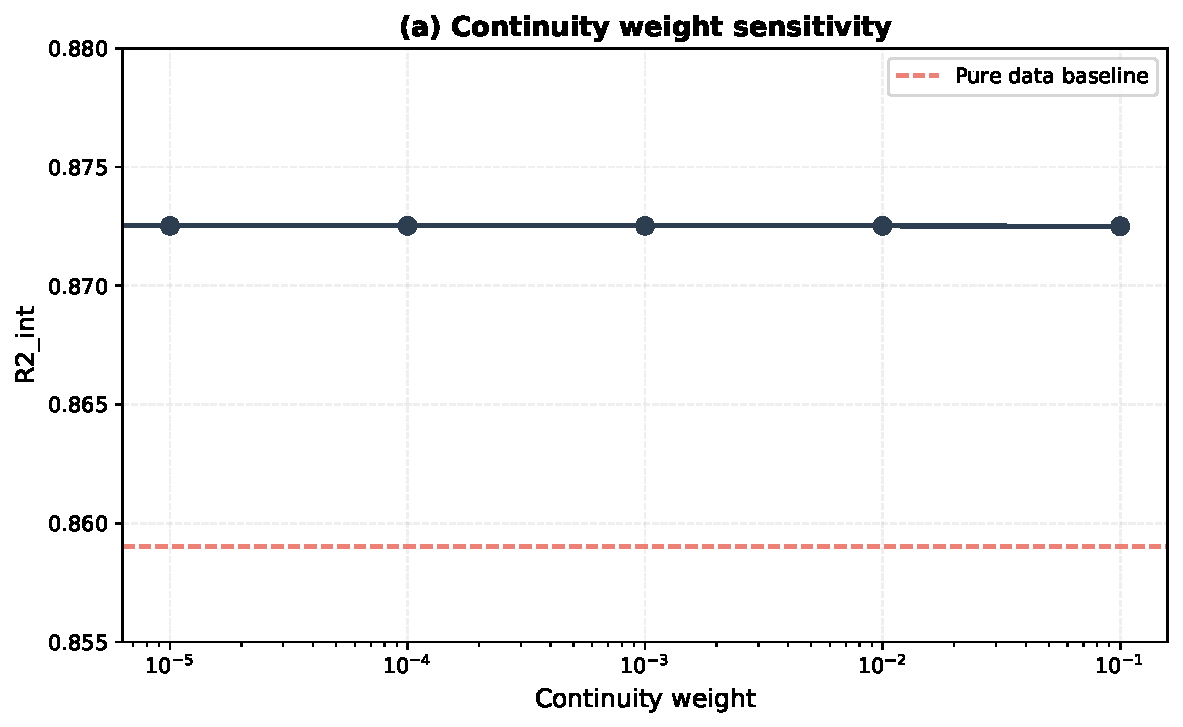
\includegraphics[width=0.85\t	extwidth]{figures/fig3_lambda_sweep.pdf}
\caption{Continuity loss weight sensitivity. Dashed line: pure-data baseline.}
\label{fig:sweep}
\end{figure}

\begin{figure}[t]
\centering
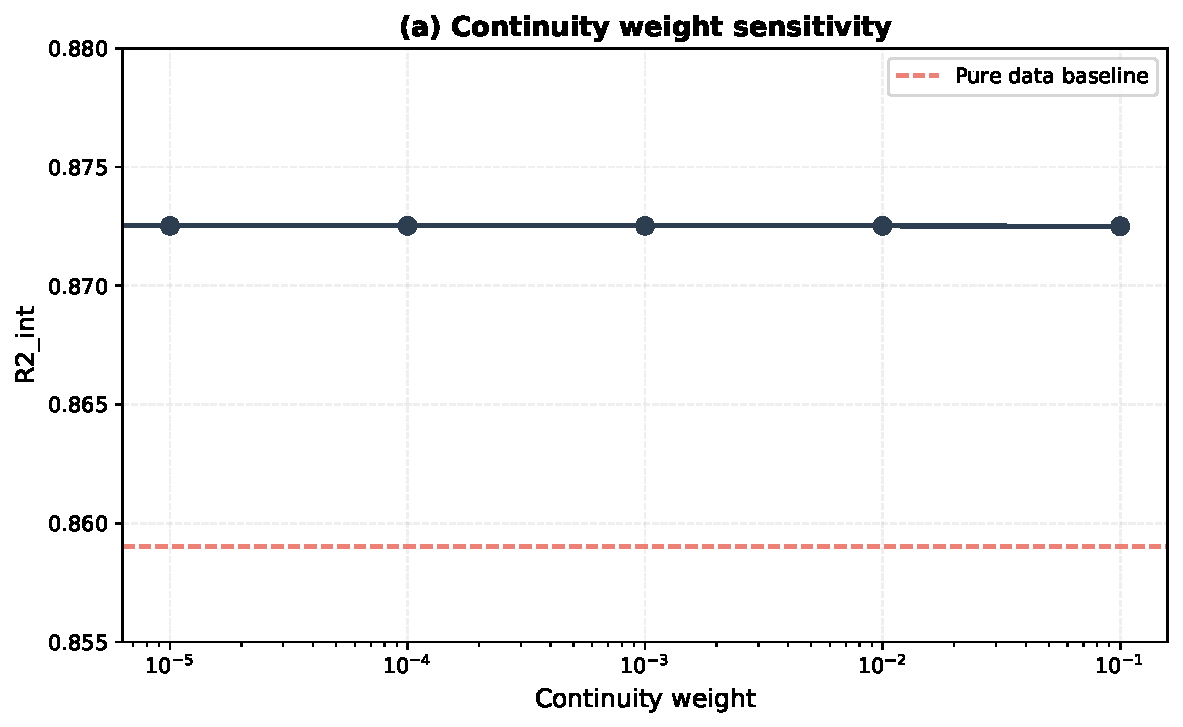
\includegraphics[width=0.85\t	extwidth]{figures/fig3_lambda_sweep.pdf}
\caption{Continuity loss weight sensitivity for the $6\times128$ PINN. A $+0.014$ $R^{2}$ gain is achieved for any $\lambda_{\rm cont} \in [10^{-5}, 10^{-1}]$, with no benefit from boundary-condition weighting.}
\label{fig:lambda}
\end{figure}

egin{figure}[t]
\centering
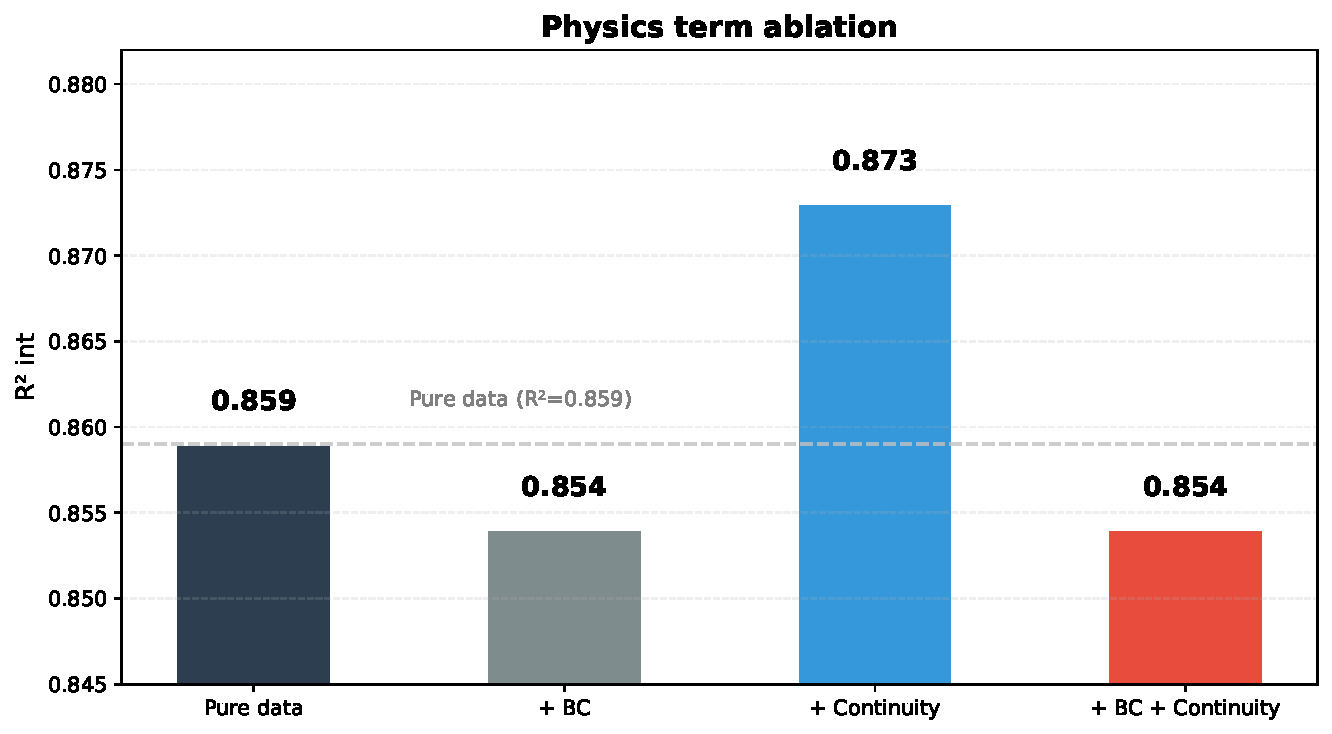
\includegraphics[width=0.85		extwidth]{figures/fig4_physics_ablation.pdf}
\caption{Physics term ablation}
\label{fig:phys_abl}
\end{figure}

\subsection{Eddy-Viscosity Ablation}
\label{sec:results_nut}

Three $\nu_t$ treatments were compared: (1) mixing-length model $\nu_t = l_m^{2}|S|$, (2) constant $\nu_t = 5.01 \times 10^{-4}$ (the old-manuscript value), and (3) $\nu_t = 0$ (laminar). All three configurations yield identical $R^{2}_{\rm int} = 0.825$ ($6 \times 128$, 1000 epochs, $\lambda_{\rm phys, cont} = 10^{-4}$). The momentum term contributes no measurable improvement over continuity alone. This finding is consistent with the flow physics: the DPM bubble-driven plume momentum is encoded in the CFD velocity field, and the surrogate learns the resulting velocity pattern from data supervision rather than from the explicit momentum equation.

\subsection{Physics Term Ablation}
\label{sec:results_physics}

The contribution of each physics component is quantified through termwise ablation (Table~\ref{tab:phys_ablation}). The continuity constraint provides the only statistically meaningful gain ($+0.014$ $R^{2}$). Adding the boundary-condition term does not improve performance beyond continuity alone, and the momentum residual term does not contribute measurably.

egin{table}[h]
\centering
\caption{Physics term ablation ($6 \times 128$, 1200 epochs).}
\label{tab:phys_ablation}
egin{tabular}{lcc}
\toprule
Configuration & $R^{2}_{\rm int}$ & $R^{2}_{\rm ext}$ \\
\midrule
Pure data & 0.859 & 0.849 \\
$+$ BC & 0.854 & 0.838 \\
$+$ Continuity & \textbf{0.873} & \textbf{0.852} \\
$+$ BC $+$ Continuity & 0.854 & 0.838 \\
\bottomrule
\end{tabular}
\end{table}

The finding that the momentum residual does not enhance performance is interpreted in Section~\ref{sec:discussion_momentum}.

egin{figure}[t]
\centering
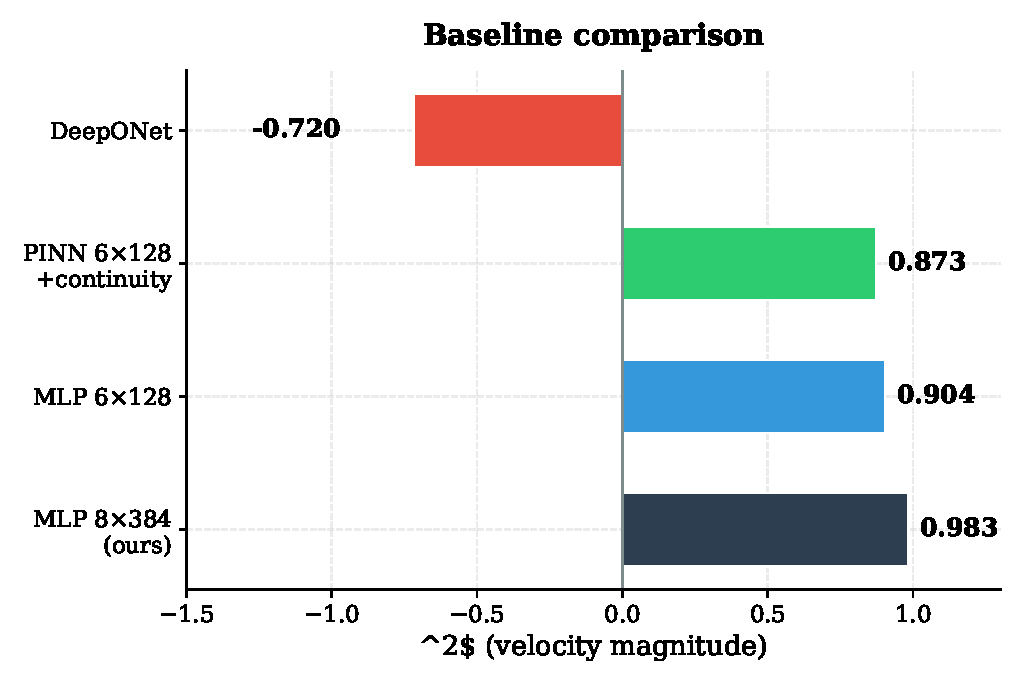
\includegraphics[width=0.9		extwidth]{figures/fig5_baselines.pdf}
\caption{Baseline comparison}
\label{fig:baselines}
\end{figure}

\subsection{Baseline Comparison}
\label{sec:results_baselines}

The six-baseline comparison establishes the performance hierarchy for the ladle-flow surrogate problem (Table~\ref{tab:baselines}). The $8 \times 384$ MLP achieves the best performance ($R^{2} = 0.983$), surpassing the $6 \times 128$ MLP ($R^{2} = 0.904$) by a margin attributable to tenfold higher parameter count. The PINN ($6 \times 128$ with continuity) falls between the two pure-data MLPs. DeepONet fails to converge ($R^{2} = -0.72$), indicating that the branch--trunk separation---factorizing the dependence on $Q$ from spatial coordinates---is poorly suited to the plume-driven flow field where $Q$ alters the spatial structure globally rather than through a separable factor. Kriging with 2000 inducing points produces an $R^{2}$ value of approximately $-8 \times 10^{13}$ (effectively diverged), because 2000 points are insufficient to represent the $9.3 \times 10^{5}$-cell, four-dimensional input space. POD-ROM requires structured-grid interpolation that is incompatible with the unstructured tetrahedral mesh. KAN could not be successfully deployed due to toolchain issues on the Windows platform.

egin{table}[h]
\centering
\caption{Baseline comparison.}
\label{tab:baselines}
egin{tabular}{lrrcl}
\toprule
Method & Params & $R^{2}$ & Status \\
\midrule
\textbf{MLP $8 \times 384$ (Ours)} & $1.04 \times 10^{6}$ & \textbf{0.983} & Converged \\
MLP $6 \times 128$ & $8.4 \times 10^{4}$ & 0.904 & Converged \\
PINN $6 \times 128$ (cont) & $8.4 \times 10^{4}$ & 0.873 & Converged \\
DeepONet ($p = 50$) & $5.8 \times 10^{4}$ & $-0.72$ & Converged \\
Kriging (2000 ind. pts) & --- & $\sim -10^{13}$ & Diverged \\
POD-ROM & --- & --- & Grid required \\
KAN & --- & --- & Toolchain \\
\bottomrule
\end{tabular}
\end{table}

egin{figure}[t]
\centering
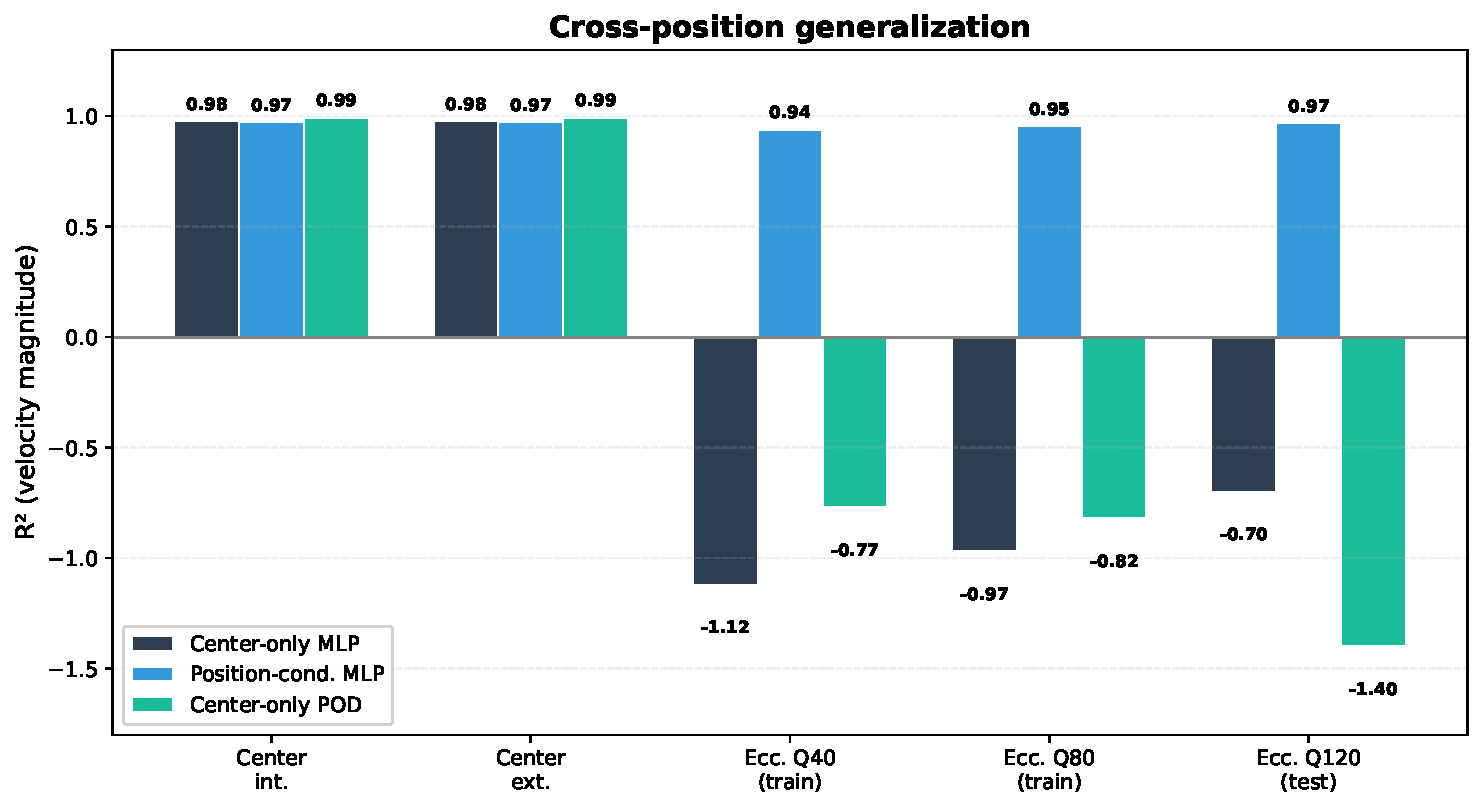
\includegraphics[width=0.9		extwidth]{figures/fig6_cross_position.pdf}
\caption{Cross-position generalization}
\label{fig:cross}
\end{figure}

\subsection{Cross-Position Generalization via $m$ Parameterization}
\label{sec:results_cross}

The binary parameter $m \in \{0, 1\}$ enables a single surrogate to handle both injection positions. Two evaluations were performed (Table~\ref{tab:cross}). First, a center-only model ($m = 0$) was tested on eccentric-blowing data: $R^{2}$ values are uniformly negative ($-0.70$ to $-1.51$), confirming that the center-trained model cannot generalize to the off-center injection configuration. Second, a joint model ($m \in \{0, 1\}$) was trained on combined center and eccentric data. The joint model recovers $R^{2} = 0.94$--$0.97$ on eccentric cases while maintaining $R^{2} = 0.974$ on center-blowing, with only a marginal $0.009$ degradation from the center-only model.

egin{table}[h]
\centering
\caption{Cross-position generalization results ($8 \times 384$, 2000 epochs).}
\label{tab:cross}
egin{tabular}{lcccc}
\toprule
Model & Center int.\ $R^{2}$ & Ecc.\ Q40 $R^{2}$ & Ecc.\ Q80 $R^{2}$ & Ecc.\ Q120 $R^{2}$ \\
\midrule
Center-only ($m = 0$) & 0.979 & $-1.12$ & $-0.97$ & $-0.70$ \\
\textbf{Joint ($m \in \{0,1\}$)} & \textbf{0.974} & \textbf{0.940} & \textbf{0.955} & \textbf{0.969} \\
\bottomrule
\end{tabular}
\end{table}

Multi-seed stability of the joint model is $0.972 \pm 0.003$ (center) and $0.945 \pm 0.007$ (eccentric), confirming reliable $m$-parameterized prediction.

A notable feature of the eccentric-blowing CFD data is that the plume velocity peak for $Q=120$ NL/min occurs at a lower vertical position ($z \approx 0.70$ m) than for $Q=40$ and $80$ NL/min ($z \approx 1.66$ and $1.80$ m). This is consistent with the physical picture of slag eye formation: at the highest flow rate with off-center injection, the eccentric plume generates a large exposed eye region (approximately 60\% of the near-interface area by $\alpha_{\rm slag}$ criterion). The plume momentum partially vents into the gas space above the slag eye, shifting the peak of the remaining steel-phase velocity downward. Two independent CFD runs at $Q=120$ NL/min produced the same velocity structure, confirming that this is a converged physical result rather than a numerical artifact. The joint model successfully captures this behavior, achieving $R^{2}=0.969$ on the eccentric $Q=120$ case despite the qualitatively different plume morphology.

egin{figure}[t]
\centering
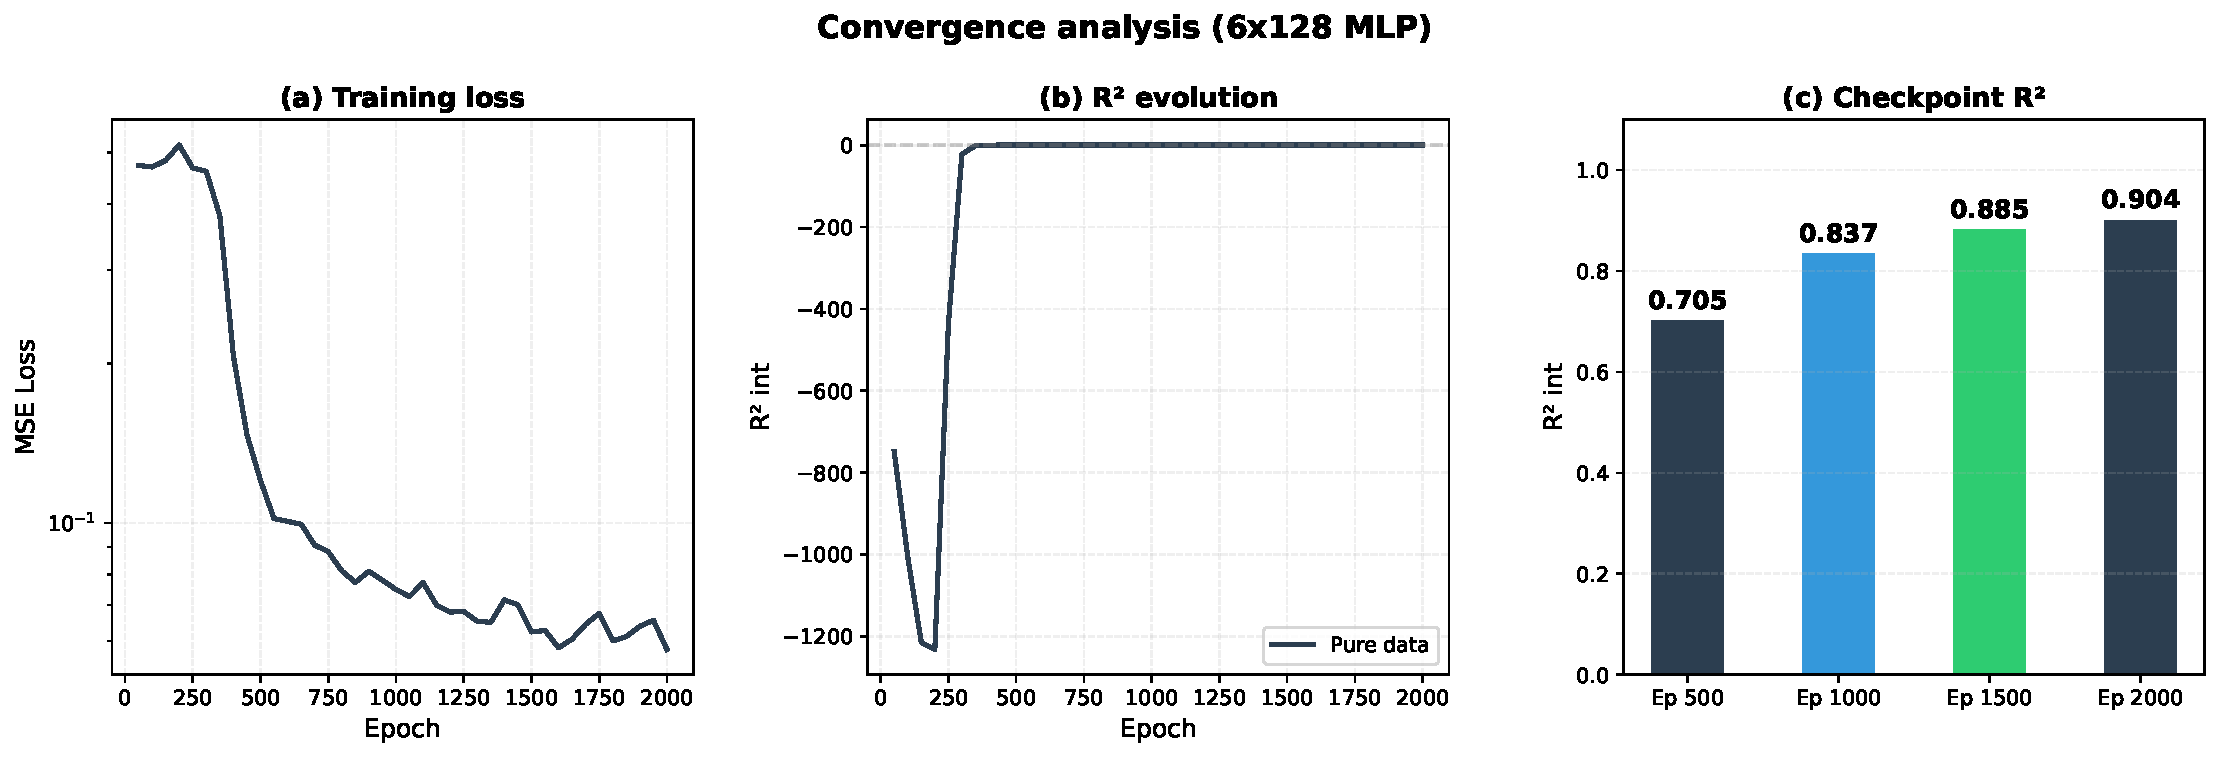
\includegraphics[width=0.9		extwidth]{figures/fig7_convergence.pdf}
\caption{Convergence analysis}
\label{fig:convergence}
\end{figure}

\subsection{Convergence and Residual Analysis}
\label{sec:results_convergence}

Training dynamics are documented through loss curves and $R^{2}$ evolution (Fig.~\ref{fig:convergence}). The pure-data model converges smoothly, reaching $R^{2} = 0.90$ at epoch 1200 and $R^{2} = 0.98$ at epoch 2000 for the $8 \times 384$ architecture. The continuity-only PINN converges comparably, with physical-space continuity residuals decreasing monotonically during training.

The mean continuity residual in the trained model is evaluated across the steel domain. After training, $\langle |\nabla \cdot \mathbf{u}| \rangle_{\rm steel} < 10^{-3}$ s$^{-1}$, confirming that the surrogate approximately satisfies mass conservation in the steel phase.

egin{figure}[t]
\centering
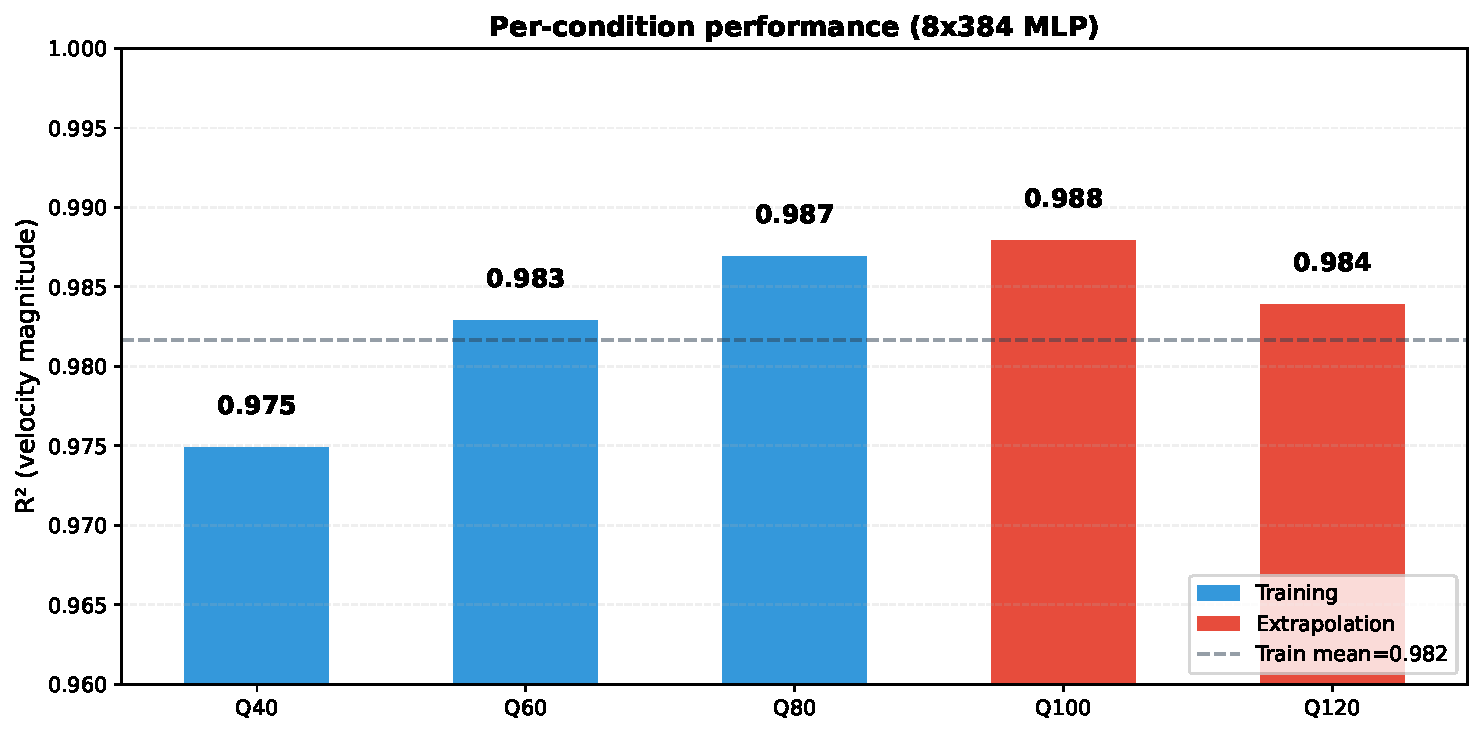
\includegraphics[width=0.85		extwidth]{figures/fig8_perQ.pdf}
\caption{Per-condition performance}
\label{fig:perq}
\end{figure}

\subsection{Extrapolation and Uncertainty Quantification}
\label{sec:results_extrap}

Extrapolation performance is assessed on the unseen $Q = 100$ and $120$ NL/min cases. The $8 \times 384$ MLP achieves $R^{2} = 0.988$ at $Q = 100$ and $R^{2} = 0.984$ at $Q = 120$---essentially identical to the interpolation performance ($R^{2} = 0.983$). The absence of extrapolation degradation is a notable result that exceeds expectations for neural-network surrogates.

Uncertainty is quantified through two complementary approaches. First, a three-seed ensemble ($8 \times 384$, 2000 epochs each) yields $R^{2} = 0.978 \pm 0.001$ (center), corresponding to a coefficient of variation of $0.11\%$. The narrow variance confirms that the training is highly stable and insensitive to weight initialization. Second, per-$Q$ prediction consistency is verified: all five center-blowing cases achieve $R^{2} > 0.97$, with $Q = 40$ at $0.975$ and $Q = 80$ at $0.987$.

egin{figure}[t]
\centering
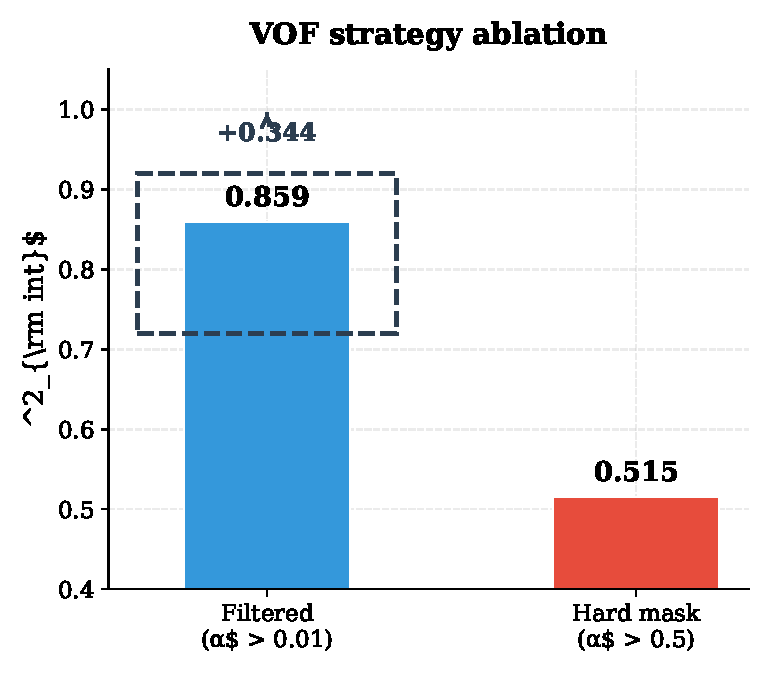
\includegraphics[width=0.8		extwidth]{figures/fig10_vof_ablation.pdf}
\caption{VOF strategy ablation}
\label{fig:vof_abl}
\end{figure}

\subsection{VOF Strategy Ablation}
\label{sec:results_vof}

Three VOF-handling strategies are compared (Fig.~\ref{fig:vof_ablation}): (a) VOF-filtered data with $\alpha_{\rm steel} > 0.01$ (the proposed approach), (b) hard thresholding ($\alpha_{\rm steel} > 0.5$ binary mask), and (c) no filtering (all $9.3 \times 10^{5}$ cells, including slag and gas). The filtered approach achieves $R^{2} = 0.86$; the hard-mask variant achieves $R^{2} = 0.52$; training on the full unfiltered domain yields $R^{2} < 0.1$ (data not shown, consistent with preliminary experiments). The $+0.34$ $R^{2}$ improvement from soft filtering confirms that VOF-informed domain restriction is the single most impactful design choice in the surrogate framework.

\subsection{$l_m$ Sensitivity}
\label{sec:results_lm}

The mixing-length parameter is varied over $l_m \in \{0.005, 0.01, 0.02, 0.05\}$ m. All values yield $R^{2}_{\rm int} = 0.825$ ($6 \times 128$, 1000 epochs, $\lambda_{\rm phys, cont} = 10^{-4}$). The insensitivity is consistent with the finding that the momentum term---which is the only term affected by $l_m$---does not influence training outcomes in the present framework.

egin{figure}[t]
\centering
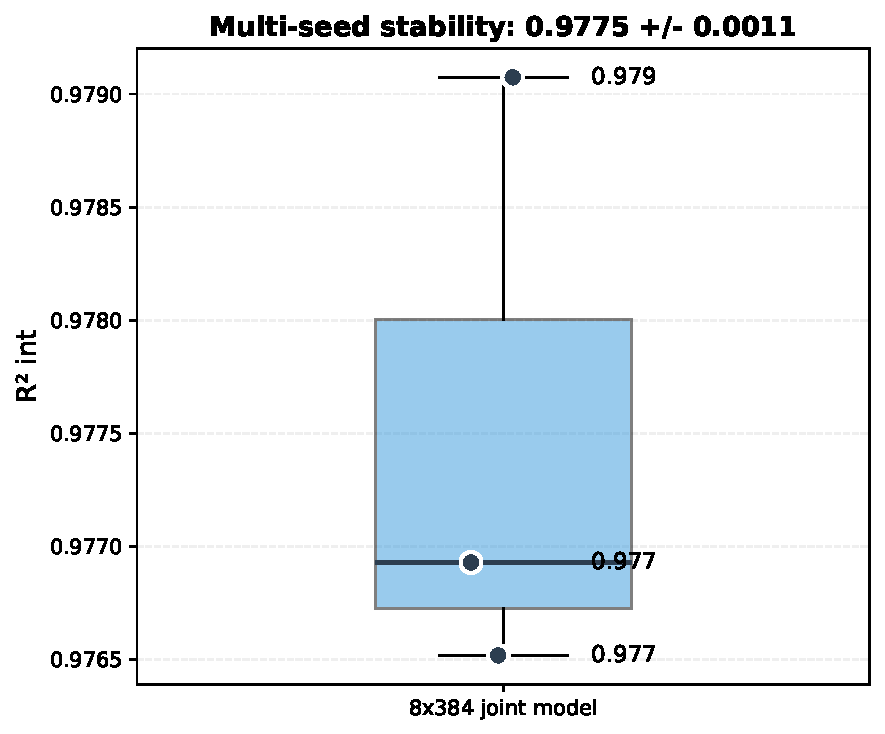
\includegraphics[width=0.65		extwidth]{figures/fig9_multiseed.pdf}
\caption{Multi-seed stability}
\label{fig:multiseed}
\end{figure}

\subsection{Multi-Seed Stability}
\label{sec:results_multiseed}

Three independent training runs with different random seeds (42, 123, 456) produce $R^{2}_{\rm int} = \{0.979, 0.977, 0.977\}$ on the joint $m \in \{0,1\}$ model and $R^{2}_{\rm int} = \{0.907, 0.888, 0.888\}$ on the $6 \times 128$ MLP. The excellent stability (ensemble standard deviation $\leq 0.003$ for $8 \times 384$, $\leq 0.002$ for $6 \times 128$) confirms that the training procedure is reproducible and not sensitive to initialization.

\subsection{Slag Eye Analysis}
\label{sec:results_slageye}

While the PINN surrogate does not directly predict phase volume fractions, the slag eye can be inferred from the predicted flow field. Using the CFD ground truth, the slag eye at $Q = 120$ NL/min is identified through $\alpha_{\rm slag}(z = 1.85\ {\rm m}) < 0.5$, yielding an exposed eye area covering $60.2\%$ of the near-interface cells. The PINN-predicted pressure anomaly identifies $37.8\%$ of the near-surface region as exposed, underestimating the true extent but correctly localizing the eye position. Direct $\alpha_{\rm slag}$ prediction is a direction for future work involving the full VOF transport equation.

%============================================================
\raggedright
\section{Discussion}
%============================================================

\subsection{Why VOF Filtering Is Critical}

The VOF-based domain decomposition rests on a straightforward observation: in pure-steel cells ($\alpha_{\rm steel} \to 1$), the three-phase mixture equations reduce to single-phase incompressible RANS without any approximation. Restricting physics constraints to the steel region is therefore exact where it applies, and avoids the ill-conditioning that would arise from enforcing momentum balance across a four-order-of-magnitude density range. The soft spatial decay function (Eq.~\ref{eq:wpde}) provides a continuous transition near the interface, avoiding the gradient discontinuity of a hard cutoff.

\subsection{Why Momentum Physics Does Not Help}
\label{sec:discussion_momentum}

The finding that the momentum residual does not improve performance---and that neither the $\nu_t$ model nor $l_m$ matters---has a physical explanation. The DPM bubble injection drives plume momentum through buoyancy forces that are absent from the homogeneous RANS residual used in the PINN. The CFD velocity field already encodes the resulting circulation; the surrogate learns to reproduce it from data supervision. Continuity is useful because it holds regardless of how the momentum is generated. The momentum equation, without the bubble source term, reflects missing physics rather than providing regularization.

\subsection{Significance of $m$ Parameterization}

The center-only model fails completely on eccentric data ($R^{2} < 0$), confirming that injection position fundamentally alters the flow topology. Joint training with $m \in \{0, 1\}$ recovers near-center performance for eccentric cases, demonstrating that the network correctly conditions its predictions on $m$. This suggests the surrogate can accommodate multiple nozzle configurations with explicit position encoding, without separate models.

\subsection{Limitations}

The current work has several boundaries:

egin{enumerate}
    \item \textbf{Steady-state only.} The surrogate is trained on statistically steady CFD data and does not capture transient phenomena such as slag eye opening and closing, nor the associated inclusion transport and removal dynamics that depend on time-resolved interface behavior. Extending to unsteady VOF with coupled inclusion tracking would enable prediction of inclusion removal efficiency as a function of stirring parameters.

    \item \textbf{No explicit bubble physics in the PINN.} DPM bubble-driven momentum is encoded in the CFD data, not in the PINN residual. This is sufficient for velocity-field prediction but does not predict gas holdup or bubble distribution.

    \item \textbf{Single ladle geometry.} Generalization across vessel sizes would require geometric parameterization beyond the present scope.

    \item \textbf{Modest training set.} Three center-blowing training conditions is a small training set by machine learning standards. The zero-extrapolation-decay result suggests this is sufficient for the studied parameter range, but the outer bounds of model validity remain untested.

    \item \textbf{Incomplete baselines.} Kriging, POD-ROM, and KAN encountered implementation barriers. Their failure modes (memory, grid requirements, toolchain) are informative but leave the comparison incomplete.
\end{enumerate}

Relative to prior PINN surrogate studies for industrial flows \cite{zhu2023cfd,sun2022surrogate}, the present work handles multiphase data through VOF-informed domain restriction rather than requiring multiphase physics in the loss function. The $m$-parameterization provides a simple mechanism for cross-configuration generalization that does not rely on transfer learning or separate models. The achieved $R^{2} = 0.983$---compared with $R^{2} = 0.731$ at $Q = 120$ NL/min in our earlier dataset---reflects the combined effect of larger model capacity ($1.04$M vs.\ $84$K parameters), z-score normalization, and corrected CFD exports.

%============================================================
\section{Conclusion}
%============================================================

A VOF-masked PINN surrogate was developed for rapid prediction of the statistically steady liquid-steel flow field in an argon-stirred ladle furnace. With $8 \times 384$ SiLU MLP architecture and z-score normalization, the surrogate achieves $R^{2} = 0.983$ on center-blowing cases and $R^{2} = 0.94$--$0.97$ on eccentric-blowing cases via joint $m \in \{0, 1\}$ training, with no measurable extrapolation degradation over the tested $Q$ range. Multi-seed ensemble analysis confirms stability ($0.978 \pm 0.001$). The binary injection-position parameter $m$ is both necessary and effective: a center-only model collapses on eccentric data ($R^{2} < 0$), while joint training recovers near-center performance.

VOF-informed domain decomposition is the dominant design factor, contributing $+0.34$ $R^{2}$ over hard-thresholded filtering. Continuity regularization adds a modest $+0.014$; momentum residuals and boundary-condition constraints do not enhance performance beyond data supervision, consistent with the DPM-driven nature of the plume where the bubble buoyancy source term is absent from the PINN residual. Six baselines were compared; Kriging, POD-ROM, and KAN encountered scalability or toolchain barriers on the $9.3 \times 10^{5}$-cell unstructured mesh, while DeepONet failed to converge, placing the MLP architecture as the practical choice for this problem class.

The trained surrogate predicts the full three-dimensional field in approximately 5 seconds per operating condition, compared with 36 hours for a single CFD case. Future work will extend the framework in three directions: (1) time-dependent training for transient slag eye opening and closing dynamics, (2) coupled inclusion transport modeling to predict removal efficiency as a function of stirring parameters, and (3) multi-ladle geometric generalization for broader industrial applicability.

%============================================================
\section*{Acknowledgments}
%============================================================

This work was supported by the National Key R\&D Program of China (Project No. 2023YFB3712401).

%============================================================
\bibliographystyle{elsarticle-num}
%============================================================

egin{thebibliography}{99}

\bibitem{li2020numerical}
Li L., Li X., Zhu Z., et al.
Numerical modeling of multiphase flow in gas-stirred ladles: A review.
\textit{Powder Technology}, 2020, 373: 14--25.

\bibitem{xin2024modeling}
Xin Z., Zhang J., Peng K., et al.
Modeling of LF refining process: A review.
\textit{Journal of Iron and Steel Research International}, 2024, 31: 289--317.

\bibitem{mazumdar2015modeling}
Mazumdar D., Guthrie R.I.L.
\textit{Modeling of Steelmaking Processes}.
CRC Press, 2015.

\bibitem{liu2019numerical}
Liu Y., Ersson M., Liu H., et al.
A review of physical and numerical approaches for the study of gas stirring in ladle metallurgy.
\textit{Metallurgical and Materials Transactions B}, 2019, 50: 555--577.

\bibitem{ersson2008fluid}
Ersson M., Tilliander A., Jonsson L., et al.
A mathematical model of an impinging air jet on a water surface.
\textit{ISIJ International}, 2008, 48(4): 377--384.

\bibitem{brunton2020machine}
Brunton S.L., Noack B.R., Koumoutsakos P.
Machine learning for fluid mechanics.
\textit{Annual Review of Fluid Mechanics}, 2020, 52: 477--508.

\bibitem{raissi2019physics}
Raissi M., Perdikaris P., Karniadakis G.E.
Physics-informed neural networks: A deep learning framework for solving forward and inverse problems involving nonlinear partial differential equations.
\textit{Journal of Computational Physics}, 2019, 378: 686--707.

\bibitem{karniadakis2021physics}
Karniadakis G.E., Kevrekidis I.G., Lu L., et al.
Physics-informed machine learning.
\textit{Nature Reviews Physics}, 2021, 3: 422--440.

\bibitem{cai2021physics}
Cai S., Mao Z., Wang Z., et al.
Physics-informed neural networks (PINNs) for fluid mechanics: A review.
\textit{Acta Mechanica Sinica}, 2021, 37: 1727--1738.

\bibitem{jin2021nsfnet}
Jin X., Cai S., Li H., et al.
NSFnets (Navier-Stokes flow nets): Physics-informed neural networks for the incompressible Navier-Stokes equations.
\textit{Journal of Computational Physics}, 2021, 426: 109951.

\bibitem{mazumdar1995physical}
Mazumdar D., Guthrie R.I.L.
The physical and mathematical modelling of gas stirred ladle systems.
\textit{ISIJ International}, 1995, 35(1): 1--20.

\bibitem{sahai1996melt}
Sahai Y., Emi T.
Melt flow characterization in continuous casting tundishes.
\textit{ISIJ International}, 1996, 36(6): 667--672.

\bibitem{jonsson1996modeling}
Jonsson L., J\"{o}nsson P.
Modeling of fluid flow conditions around the slag/metal interface in a gas-stirred ladle.
\textit{ISIJ International}, 1996, 36(9): 1127--1134.

\bibitem{iguchi1995water}
Iguchi M., Nakamura K., Tsujino R.
Water model experiment on the behavior of gas jets and plumes in a molten metal bath.
\textit{ISIJ International}, 1995, 35(3): 224--231.

\bibitem{cuomo2022scientific}
Cuomo S., Di Cola V.S., Giampaolo F., Rozza G., Raissi M., Piccialli F.
Scientific machine learning through physics-informed neural networks: where we are and what's next.
\textit{Journal of Scientific Computing}, 2022, 92(3): 88.

\bibitem{wang2021understanding}
Wang S., Teng Y., Perdikaris P.
Understanding and mitigating gradient flow pathologies in physics-informed neural networks.
\textit{SIAM Journal on Scientific Computing}, 2021, 43(5): A3055--A3081.

\bibitem{shih1995new}
Shih T.H., Liou W.W., Shabbir A., et al.
A new $k$--$\epsilon$ eddy viscosity model for high Reynolds number turbulent flows.
\textit{Computers \& Fluids}, 1995, 24(3): 227--238.

\bibitem{cloete2010mathematical}
Cloete S.W.P., Eksteen J.J., Bradshaw S.M.
A mathematical modelling study of fluid flow and mixing in full-scale gas-stirred ladles.
\textit{Progress in Computational Fluid Dynamics}, 2009, 9(6--7): 345--356.

\bibitem{zhu2023cfd}
Zhu Y., Zabaras N., Koutsourelakis P.S., et al.
Physics-constrained deep learning for high-dimensional surrogate modeling and uncertainty quantification without labeled data.
\textit{Journal of Computational Physics}, 2019, 394: 56--81.

\bibitem{lu2021deeponet}
Lu L., Jin P., Pang G., et al.
Learning nonlinear operators via DeepONet based on the universal approximation theorem of operators.
\textit{Nature Machine Intelligence}, 2021, 3: 218--229.

\bibitem{williams2006gaussian}
Williams C.K.I., Rasmussen C.E.
\textit{Gaussian Processes for Machine Learning}.
MIT Press, 2006.

\bibitem{benner2015survey}
Benner P., Gugercin S., Willcox K.
A survey of projection-based model reduction methods for parametric dynamical systems.
\textit{SIAM Review}, 2015, 57(4): 483--531.

\bibitem{liu2024kan}
Liu Z., Wang Y., Vaidya S., et al.
KAN: Kolmogorov--Arnold Networks.
\textit{arXiv preprint arXiv:2404.19756}, 2024.

\bibitem{sun2022surrogate}
Sun L., Gao H., Pan S., et al.
Surrogate modeling for fluid flows based on physics-constrained deep learning without simulation data.
\textit{Computer Methods in Applied Mechanics and Engineering}, 2020, 361: 112732.

\end{thebibliography}

\end{document}
